\chapter{Previous and Related Work}
\label{ch:related_work}
This chapter outlines work done by other people related to my problem description. It has two main sections: the first part describes existing frameworks for creating state machine -based systems, and the second part outlines some previous attempts at working with Lua in embedded systems. I have not been able to find any previous work combining the two topics, so I will assume it is a fairly untouched field.

\section{Existing Frameworks for State Machine Applications}
\label{sec:existing_frameworks_state_machine}
State machine -based systems is a well-established concept in the world of software, and several frameworks already exist for developing applications based on this concept. These frameworks vary in implementation language, design method and portability, and some of their main properties will be outlined in this section. These frameworks will be used for comparison when evaluating Lua/eLua for state machine -based systems.

\subsection{Reactive Blocks}
\label{sec:reactive_blocks}
Reactive Blocks\footnote{\url{http://www.bitreactive.com}} is a Java-based framework for developing state machine applications. It offers integration with the Eclipse \gls{ide}, and is essentially a code/application generator with a graphical interface, tailored for event-driven and concurrent systems. Application design is done by creating, connecting and combining various \emph{building blocks}. These building blocks consist of three parts:
\begin{itemize}
	\item Activity diagram: describes the internal behavior and logic of the block.
	\item External state machine: serves as an interface towards other blocks and the enclosing application. Defines which input signals are allowed in a given state, transitions associated with an input signal and a state, and any output signals resulting from the transition.
	\item Java methods that handle any operations performed as part of a transition.
\end{itemize}

An example of a building block in Reactive Blocks is displayed in Fig.~\ref{figure:reactive_blocks}.

\begin{figure}[h]
	\centering
	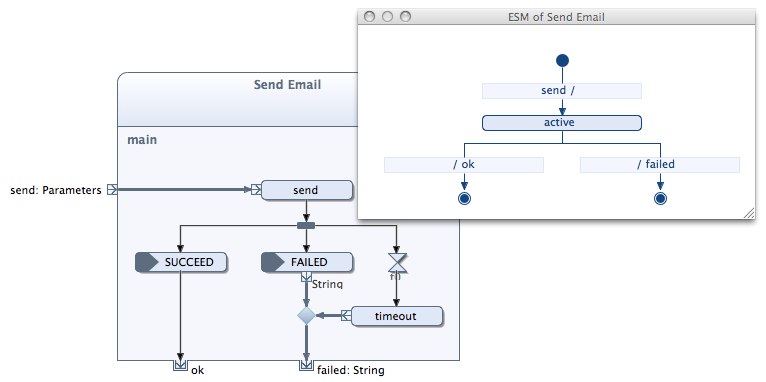
\includegraphics[scale=0.5]{reactive_blocks}
	\caption[A building block in Reactive Blocks]{An example of a building block in Reactive Blocks, displaying the activity diagram (to the left) and the external state machine (to the right). Image source: \url{http://reference.bitreactive.com/doc/building_blocks} \label{figure:reactive_blocks} }
\end{figure}

The Reactive Blocks SDK has various advantages for development of state machine -based applications:
\begin{itemize}
	\item It comes with a built-in verification tool that helps the user discover and handle logical mistakes and design flaws in the application. The framework also integrates with JUnit, for testing separate components and operations.
	\item Instead of a large and complex code base, the application consists of a hierarchy of connected building blocks, with functionality and logic defined at the design level. This generally makes projects easier to organize, maintain and extend.
	\item With the built-in runtime support system and implementation at the design level, concepts like forking, waiting and synchronization are simple, making creation of concurrent systems almost a triviality.
	\item Java has a huge base of libraries that may be combined with Reactive Blocks to provide functionality and application development on higher levels.
\end{itemize}

However, one fundamental disadvantage is that any applications created with Reactive Blocks require a Java virtual machine. This creates an obstacle when working on embedded systems, because the Java SE Embedded \gls{vm} currently only supports the \emph{most powerful} embedded systems~\cite{website:java_embedded_vm}. Memory requirements range from 130KB \gls{ram}/350KB \gls{rom} (minimal configuration) to several MB for both \gls{ram} and \gls{rom} (full configuration), which is more than what you can expect to find in a typical lightweight embedded system.

\subsection{RKH}
\label{sec:rkh_state_machine}
RKH\footnote{\url{http://rkh-reactivesys.sourceforge.net}} is a C-based development tool for implementing state machine -based systems. It is specifically designed to work on embedded systems, and consists of various platform-independent modules. The software provides a cooperative scheduler, timer and event managers, as well as a graphical interface to help designing state machines based on UML state tables. Like Reactive Blocks, RKH generates and compiles code that can be run directly. An example of a transition table statement in RKH is displayed in Fig.~\ref{figure:rkh_transition}.

\begin{figure}[h]
	\centering
	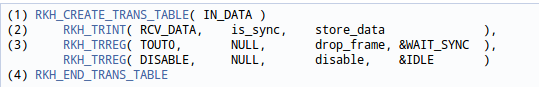
\includegraphics[scale=0.7]{rkh_transition_table}
	\caption[A transition table statement in RKH]{An example of a transition table statement in RKH, written in C code. Each line in the statement defines a transition with input signal, guard function, action function and target state. Image source: \url{http://rkh-reactivesys.sourceforge.net/qref.html} \label{figure:rkh_transition} }
\end{figure}

RKH has some particularly strong advantages when developing state machine -based applications on embedded systems:
\begin{itemize}
\item RKH is fairly platform-independent, and already built to support many platforms and processors (linux, \gls{rtos}, mbed etc…). Additionally, the modules are customizable and the project is open source, meaning it can be adapted also to custom platforms.
\item The system has a very small memory footprint, making it usable also for minimal embedded systems.
\item Application design with state tables and diagrams is simple and maintainable.
\end{itemize}

However, for the less experienced programmer, RKH also provides some challenges:
\begin{itemize}
	\item While parts of the RKH interface can be intuitively understood, other parts (like declaring actions) require at least basic knowledge of C programming. Programming in C is considered complex and difficult compared to ``higher level''-languages like Java, Python or Lua.
	\item Customization and adaptation of the software platform requires knowledge of and skills in C programming.
	\item External libraries implementing functionality are fairly limited in C, and must in some cases be adapted to the relevant platform anyway. This means C programming and extra work is required for anything but standard state machine functionality.
\end{itemize}

\subsection{Quantum Leaps}
\label{sec:quantum_leaps}
Quantum Leaps\footnote{\url{http://www.state-machine.com}} offers a product for developing state machine -based applications in two parts: an active object framework, \gls{qp}, and a graphical modeling tool, \gls{qm}.

\gls{qp} is open-source, portable, C/C++ based, and built on a non-blocking, run-to-completion kernel. \gls{qp}-applications consist of strictly encapsulated and asynchronously communicating active objects similar to the building blocks of Reactive Blocks described in Section \ref{sec:reactive_blocks}. The behavior of an active object is specified by an UML statechart, which can be modeled in \gls{qm}. QM is a fully graphical modeling environment which generates C or C++ code according to the UML statecharts to be used with the \gls{qp} framework. An example of a statechart modeled in \gls{qm} is displayed in Fig.~\ref{figure:qm_statechart}.

Some of the advantages with \gls{qp}/\gls{qm} are:
\begin{itemize}
	\item Memory requirements for \gls{qp} are very low, and range from 2KB \gls{rom}/100B \gls{ram} (\gls{qp}-nano) to 8KB \gls{rom}/1KB \gls{ram} (\gls{qp}/C and \gls{qp}/C++).
	\item \gls{qp} is ported to a large number of platforms and processors, including ARM and AVR32 processors, Android, Free\gls{rtos} and Arduino.
	\item \gls{qp} provides automatic rule checking of the generated code.
	\item \gls{qm} offers application development and implementation at the design level.
\end{itemize}

\begin{figure}[h]
	\centering
	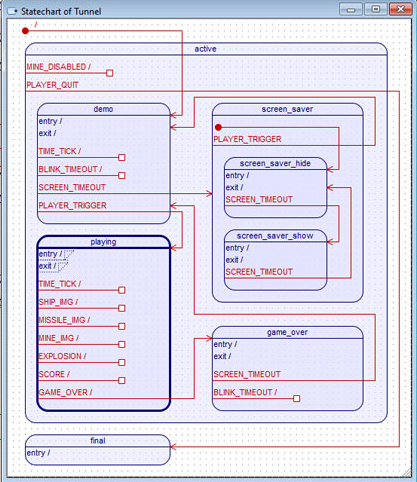
\includegraphics[scale=0.6]{qm_statechart}
	\caption[An UML statechart in QM]{A \gls{qp} active object modeled as a hierarchical UML statechart in \gls{qm}. Each statechart lists possible input signals and the following output signals or actions. Image source: \url{http://www.state-machine.com/qm/index.php} \label{figure:qm_statechart} }
\end{figure}

The major disadvantage with \gls{qp}/\gls{qm} is that it is implemented in C/C++, which means implementation of application-specific transaction operations require knowledge of C/C++ programming. However, while these are considered to be more “advanced” languages than for example Python, the level of knowledge required in this context may not be all that high (these operations can be quite simple).

\subsection{IntelliWizard}
\label{sec:intelliwizard}
\url{http://www.codeproject.com/Articles/10801/Design-State-Machine-Engine-for-embedded-system-de}
TODO

\section{Lua in Embedded Systems}
\label{sec:lua_in_embedded}
While Lua is primarily used as an extension and scripting language for applications written in other programming languages, it is also sometimes used to create standalone applications. Because of Lua's small memory footprint and configurable C source code, some effort has also been made to port the Lua interpreter to various embedded systems, both with and without the need for an underlying operating system. Some of these efforts will be outlined in this section.

\subsection{LEGO Mindstorms}
\label{sec:lego_mindstorms}
In chapter 26 of \emph{Lua Programming Gems}~\cite{chapter:porting_lua_microcontroller}, Ralph Hempel describes his efforts in porting the Lua interpreter to a platform with severe memory constraints. His choice of platform was a LEGO MINDSTORMS NXT system with an ARM7-based microcontroller, 256KB \gls{rom} and 64K \gls{ram}. Hempel, being an experienced embedded systems programmer, used his own custom toolchain for compilation and linking. The first thing he noted in the process, was that all of the changes needed to port the basic Lua code to the ARM7 microcontroller were limited to a single file, and the Lua developers had actually created a specific space for such changes. One thing requiring quite a bit of extra work, was building a \gls{rtl} to support Lua on the microcontroller (standard Lua uses libraries from the operating system). Hempel chose to build his own, but pointed out that an \gls{rtl} is usually available from the manufacturer of the system. To reduce complexity of these libraries and make it all work within the limited resources of the platform, Hempel made some changes to the capabilities of the Lua garbage collector, the I/O system, as well as the number system used (standard Lua is based only on floating-point math). His final conclusion was that while it is possible to port Lua to a microcontroller like the one he used, it requires a lot more work and consideration than simply adapting it to a different operating system.

\subsection{Einsatz von Lua in Embedded Systems}
\label{sec:einsatz_von_lua_embedded}
In their book \emph{Einsatz von Lua in Embedded Systems}\cite{book:einsatz_von_lua_embedded} (translated: ``Use of Lua in Embedded Systems''), Claus Kühnel and Daniel Zwirner explore the possibility of using Lua on various embedded platforms. Because of my limited understanding of German I have not read the entire book, but I have looked into parts of their work. Their arguments for using Lua on an embedded system include the speed/performance of the Lua interpreter, a low memory footprint (while still providing a full garbage collector), and easy interfacing with C code. Their experiments include using the Lua interpreter with libraries that control common embedded systems peripherals, as well as running Lua on actual embedded systems with limited resources, like mbed (\url{http://mbed.org/}). They also look into eLua, which is described in Section \ref{sec:elua}.

\subsection{Mihini}
\label{sec:mihini}
Mihini\footnote{\url{http://www.eclipse.org/mihini}} is an open-source embedded runtime for \gls{m2m}-applications, providing a Lua \gls{api} with the requirement of a Linux environment. In addition to the Lua \gls{api} and virtual machine, Mihini provides some useful building blocks for \gls{m2m} applications, like networking (for example their own M3DA protocol), I/O management, security, and support for some industrial protocols like Modbus. Mihini itself is not meant to run on the smallest of systems, but rather for bridging the smaller systems (like an Arduino with sensors) to the Internet. Its memory requirements are relatively small (a few MB both for \gls{rom} and \gls{ram}), which makes it suitable for systems like the Raspberry Pi. Applications for the ``slaves'' that communicate with the Mihini system are typically written in C code. Since Mihini runs on top of Linux, it is fairly trivial to port it to other platforms than the ones specified in the documentation (provided Linux is available), especially compared to the procedure described in Sect.~\ref{sec:lego_mindstorms}.

\subsection{eLua}
\label{sec:elua}
eLua\footnote{\url{http://www.eluaproject.net}} (or Embedded Lua) is an open-source, full implementation of the Lua virtual machine for some selected processors and embedded platforms. It does not require an operating system to run, and is portable to other platforms in addition to the ones supported. Like standard Lua, eLua is made to be minimalistic, and thus only offers some specific libraries for the embedded platform in addition to the standard Lua implementation. The modules are generalized and designed to run on various platform, making the Lua applications built on top of the framework almost completely platform-independent. eLua provides modules for most of the common peripherals, like LEDs, buttons, Ethernet and USB, as well as facilities like system timers and PIO. The full binary image of eLua requires ~256KB of \gls{rom}, but by removing some of the additional modules (if they are not required by the application), it can also fit on a system with only 128KB. eLua provides its own minimal file system, allowing Lua source code to be loaded onto and run directly on the microcontroller.

Because it is fairly quick and easy to get started with eLua on one of the supported platforms, I chose to use eLua with the LM3S9D92 microcontroller for my experimental work in Chapt.~\ref{ch:experimental_work}. The software provides a solid base for testing the feasibility of Lua applications, including those based on state machines, on minimalistic platforms. Some additional characteristics of eLua that are relevant in this context are described in Sect.~\ref{sec:running_on_micro}.